\section{Event Selection and Object Definitions}
\label{sec:stop_event_sel}

In this section, the definitions of the event sample and of the reconstructed
objects used in the analysis are given.

%%%%%%%%%%%%%%%%%%%%%%%%%%%%%%%%%%%%%%%%%%%%%%%%%%%%%%%%%%%%%%%%%%%%%%%%%%%%%
%%%%%%%%%%%%%%%%%%%%%%%%%%%%%%%%%%%%%%%%%%%%%%%%%%%%%%%%%%%%%%%%%%%%%%%%%%%%%
%%%%%%%%%%%%%%%%%%%%%%%%%%%%%%%%%%%%%%%%%%%%%%%%%%%%%%%%%%%%%%%%%%%%%%%%%%%%%
%
% TRIGGER
%
%%%%%%%%%%%%%%%%%%%%%%%%%%%%%%%%%%%%%%%%%%%%%%%%%%%%%%%%%%%%%%%%%%%%%%%%%%%%%
%%%%%%%%%%%%%%%%%%%%%%%%%%%%%%%%%%%%%%%%%%%%%%%%%%%%%%%%%%%%%%%%%%%%%%%%%%%%%
%%%%%%%%%%%%%%%%%%%%%%%%%%%%%%%%%%%%%%%%%%%%%%%%%%%%%%%%%%%%%%%%%%%%%%%%%%%%%

\subsection{Trigger Selection}
\label{sec:stop_trigger}

As described in Section~\ref{sec:stop_final_state}, the $W$-bosons in the three-body
\stopone decays are on-shell and therefore lead to leptons whose kinematics are not
kinematically suppressed.
Each of the leptons is expected to have similar kinematics, given the relatively uncorrelated nature
of their decay, with transverse momenta on average at the scale of $m_W / 2 \sim 40\,\GeV$.
For this reason, the analysis can rely entirely on triggers based on the leptons.
Specifically, the analysis uses the dilepton triggers listed in Table~\ref{tab:stop_triggers}.
The trigger used in each event is based on the event's dilepton flavor\footnote{The `dilepton flavor' refers to the lepton family in which each
of analysis' two leptons reside, and is indicated by two letters ($e$ or $\mu$) ordered according
to the lepton \pT. For example, a dilepton flavor of `$e\mu$' indicates an event in which the
\pT-leading lepton is an electron and the \pT-sub-leading lepton is a muon.}, since
the trigger algorithms are different for each of the three possibilities.
In data, the choice of trigger also depends on which year the data was recorded in since
the set of triggers employed in ATLAS' trigger system\footnote{The total set of triggers employed at any
given moment in ATLAS' trigger system is referred to as the `trigger menu'.}
during different data-taking years varied so as to reflect the change in data-taking conditions.

{\color{red}{Describe the anatomy of a trigger semantics in the common ana chapter}}

\begin{table}[!htb]
    \begin{center}
        \begin{tabular}{c | c | c}
          %  \toprule
            \hline
            \hline
              & \multicolumn{2}{c}{Year} \\
            Dilepton Flavor & 2015 & 2016 \\
            \hline
            $ee$  & \texttt{HLT\_2e12\_lhloose\_L12EM10VH} & \texttt{HLT\_2e17\_lhvloose\_nod0} \\
            $\mu \mu$ & \texttt{HLT\_mu18\_mu8noL1} & \texttt{HLT\_mu22\_mu8noL1} \\
            $e\mu + \mu e$ & \texttt{HLT\_e17\_lhloose\_mu14} & \texttt{HLT\_e17\_lhloose\_nod0\_mu14} \\
            \hline
            \hline
          %  \bottomrule
        \end{tabular}
        \caption{
            Triggers used in the 2015+2016 analysis searching for the \stopone quark.
        }
        \label{tab:stop_triggers}
    \end{center}
\end{table}

%%%%%%%%%%%%%%%%%%%%%%%%%%%%%%%%%%%%%%%%%%%%%%%%%%%%%%%%%%%%%%%%%%%%%%%%%%%%%
%%%%%%%%%%%%%%%%%%%%%%%%%%%%%%%%%%%%%%%%%%%%%%%%%%%%%%%%%%%%%%%%%%%%%%%%%%%%%
%%%%%%%%%%%%%%%%%%%%%%%%%%%%%%%%%%%%%%%%%%%%%%%%%%%%%%%%%%%%%%%%%%%%%%%%%%%%%
%
% OBJECT DEFINITIONS
%
%%%%%%%%%%%%%%%%%%%%%%%%%%%%%%%%%%%%%%%%%%%%%%%%%%%%%%%%%%%%%%%%%%%%%%%%%%%%%
%%%%%%%%%%%%%%%%%%%%%%%%%%%%%%%%%%%%%%%%%%%%%%%%%%%%%%%%%%%%%%%%%%%%%%%%%%%%%
%%%%%%%%%%%%%%%%%%%%%%%%%%%%%%%%%%%%%%%%%%%%%%%%%%%%%%%%%%%%%%%%%%%%%%%%%%%%%

\subsection{Object Definitions}
\label{sec:stop_object_def}

Here we describe the definitions of the leptons and jets used in the search for the
production of \stopone quarks.
The lepton (electron and muon) definitions are given in Table~\ref{tab:stop_lepton_def}
and the jet definitions are given in Table~\ref{tab:stop_jet_def}.
Discussion of the working points for lepton identification and isolation is given in
Section~\ref{sec:leptons}.
That of jets is found in Section~\ref{sec:jets} and \ref{sec:flavor_tagging}, for
jets, generically, and $b$-tagged jets, respectively.

The \pT~requirements of the leptons are such that they be on the plateau of the trigger
efficiency, {\color{red}{described in Section XXX and Figure~\ref{fig:trig_plateau_cartoon}}}.
The lepton isolation requirements are rather loose, given that a large contamination of 
fake and non-prompt leptons is not expected as a result of the requirement of two relatively
high-\pT~leptons.
The requirements on the impact parameter quantities $|d_0 / \sigma_{d_0}|$ and $|z_0 \times \sin \theta|$
further ensure that the leptons are likely to be prompt and have originated
from the primary hard-scatter vertex.

\begin{table}[!htb]
    \begin{center}
        \begin{tabular}{l | c | c | c | c }
        \hline
        \hline
            & \multicolumn{4}{c}{\textbf{Leptons}} \\
        \cline{2-5}
            & \multicolumn{2}{c}{\textbf{Electrons}} & \multicolumn{2}{c}{\textbf{Muons}} \\
        \cline{2-5}
            & \textbf{Baseline} & \textbf{Signal} & \textbf{Baseline} & \textbf{Signal} \\
        \hline
        \pT~requirement [GeV] & $(>10,>10)$ & $(>25,>20)$ & $(>10,>10)$ & $(>25,>20)$ \\
        $|\eta|$ requirement & \multicolumn{2}{c}{$<2.47$} & \multicolumn{2}{c}{$<2.4$} \\
        Identification WP & \texttt{Loose} & \texttt{Medium} & \multicolumn{2}{c}{\texttt{Medium}} \\
        Isolation & \multicolumn{4}{c}{\texttt{GradientLoose}} \\
        $|d_0 / \sigma_{d_0}|$ & $--$ & $<5$ & $--$ & $<3$ \\
        $|z_0 \times \sin \theta|$ [mm] & $--$ & $<0.5$ & $--$ & $<0.5$ \\
        \hline
        \hline
        \end{tabular}
    \end{center}
    \caption{
        Lepton definitions for the 2015+2016 analysis searching for the \stopone quark.
    }
    \label{tab:stop_lepton_def}
\end{table}

\begin{table}[!htb]
    \begin{center}
        \begin{tabular}{l | c | c}
            \hline
            \hline
                & \textbf{Jets} & \textbf{$b$-tagged Jets} \\
            \hline
            \pT~requirement [GeV] & \multicolumn{2}{c}{$>20$} \\
            $|\eta|$ requirement & $<2.8$ & $<2.4$ \\
            Pileup suppression & \multicolumn{2}{c}{ $\texttt{JVT} > 0.59$ if $\pT<60\,\GeV$~ and $|\eta| < 2.4$} \\
            Flavor-tagging WP & $--$ & $77\%$ \\
            \hline
            \hline
        \end{tabular}
    \end{center}
    \caption{
        Jet definitions for the 2015+2016 anaysis searching for the \stopone quark.
    }
    \label{tab:stop_jet_def}
\end{table}

\begin{figure}[!htb]
    \begin{center}
        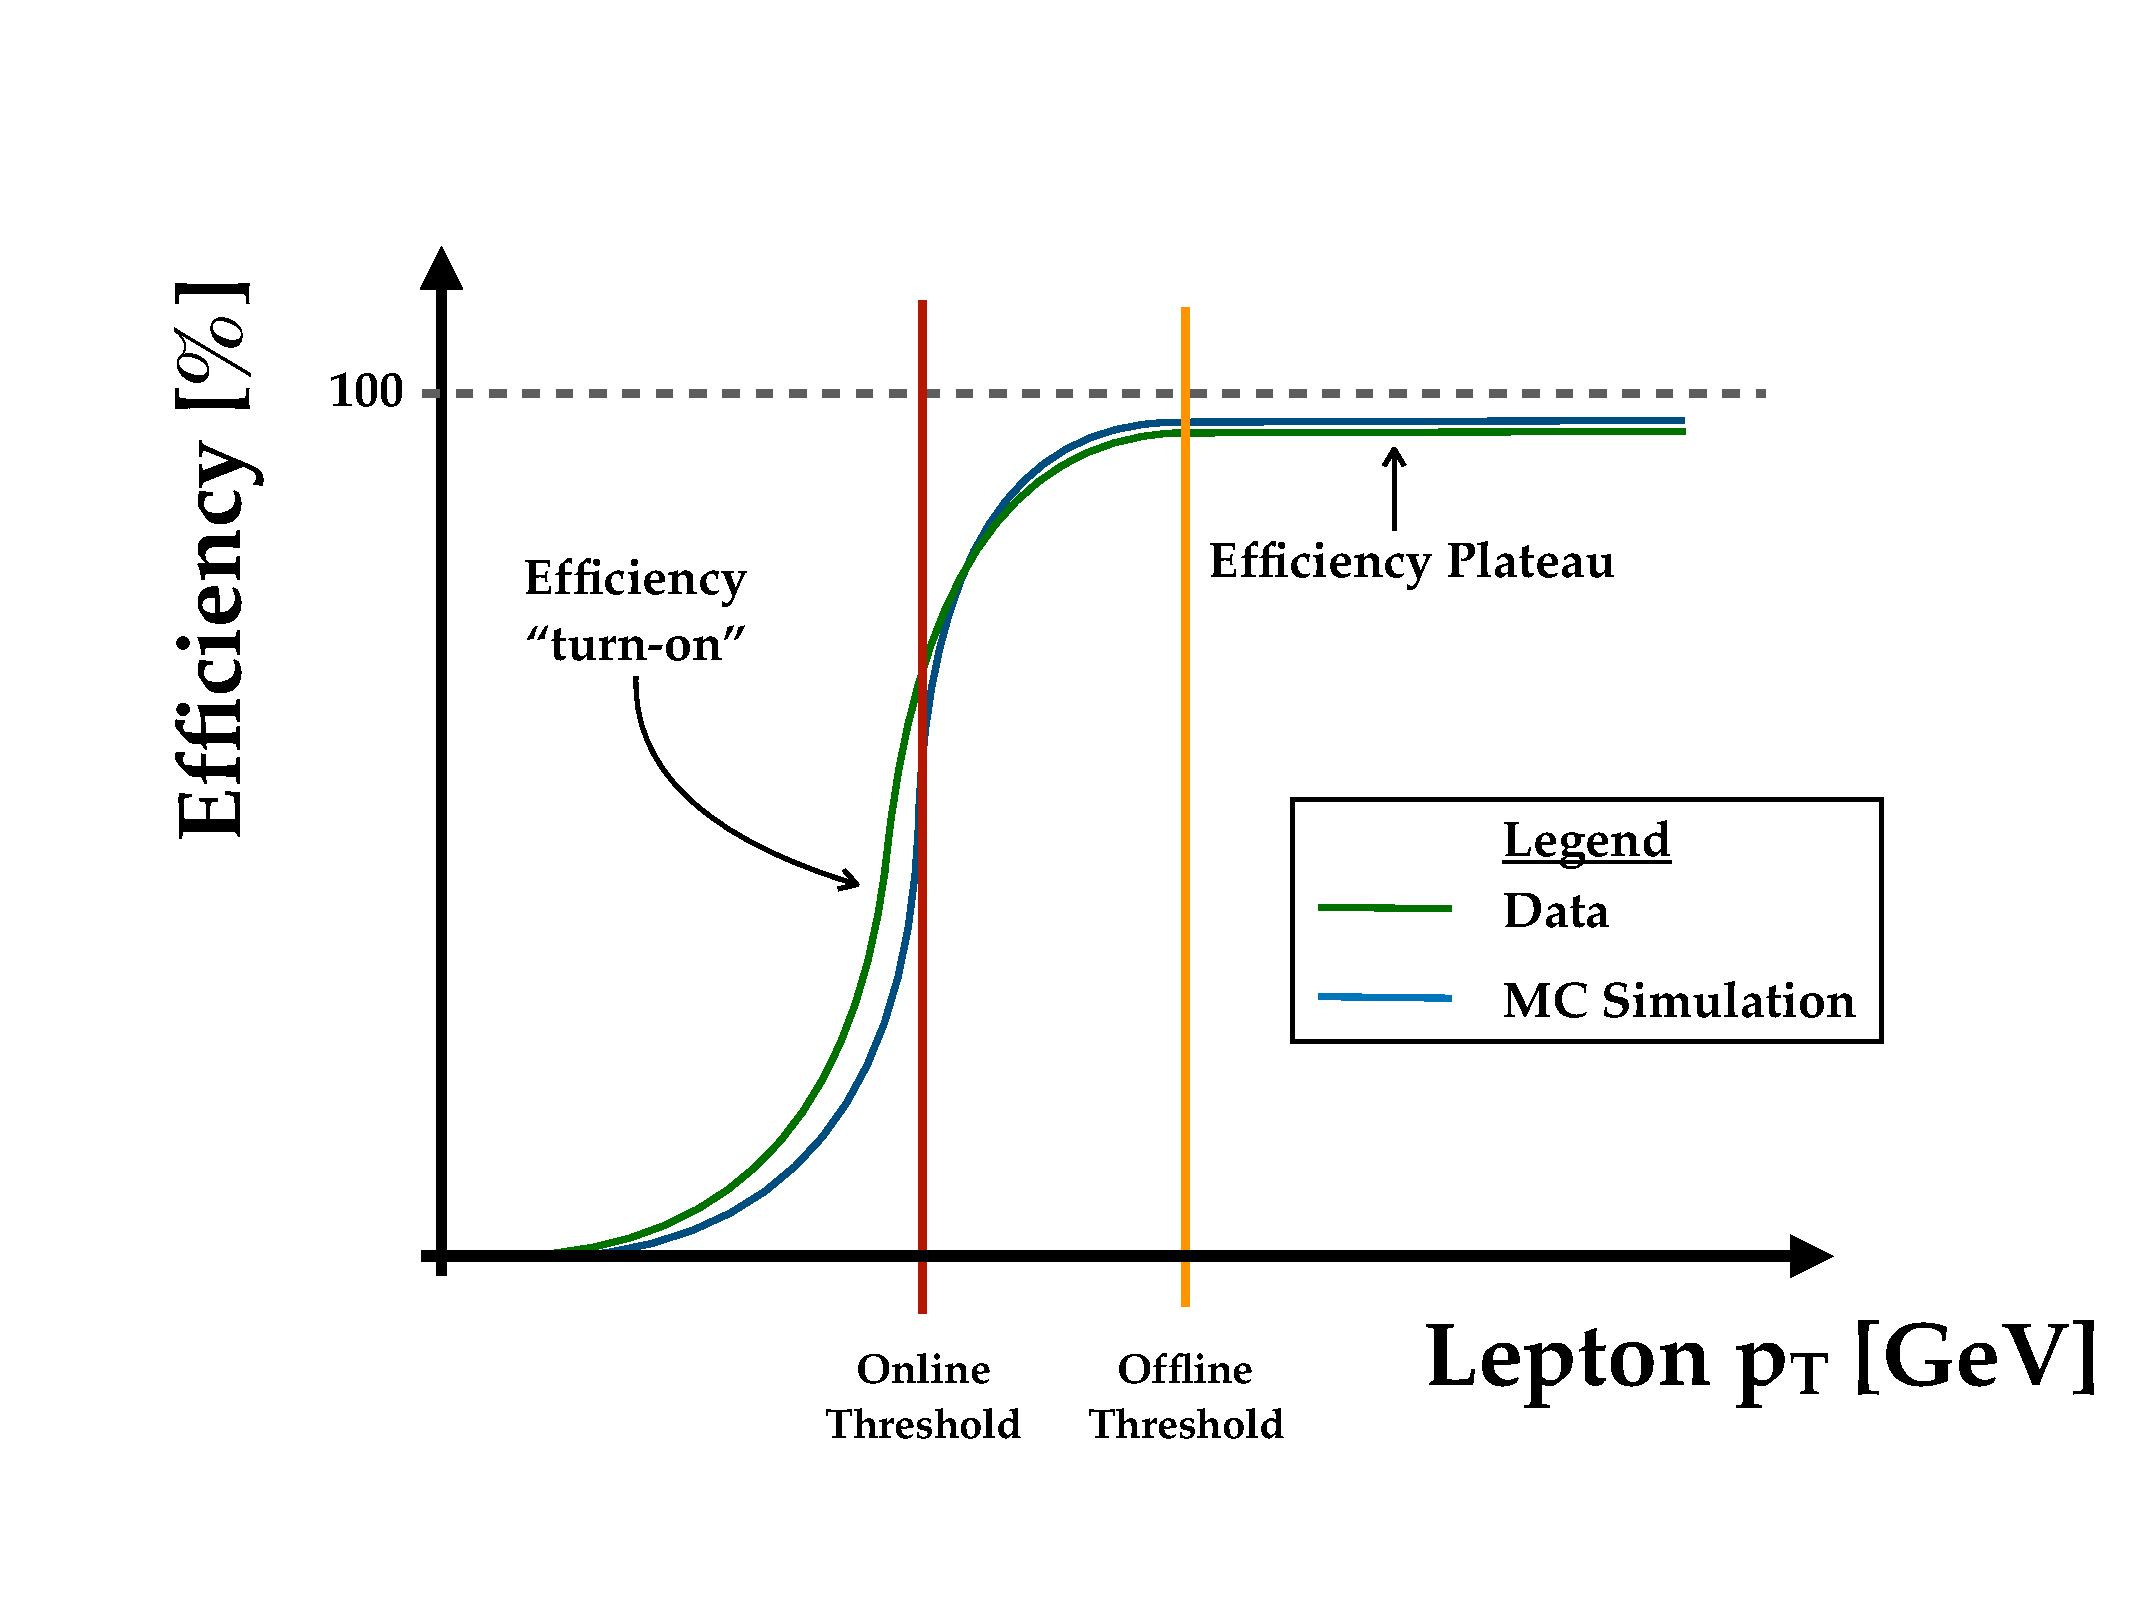
\includegraphics[width=0.75\textwidth]{figures/common_ana/trig_plateauPDF}
        \caption{
            {\color{red}{Move to common ana section on trigger, and get real example}}
            Cartoon illustrating the principle of a trigger efficiency `turn on' curve.
            The efficiency for the lepton to fire the trigger, as a function of the \pT~of the offline object, is plotted
            as a function of the offline object's \pT.
            At the online level, given the poorer lepton reconstruction resolution, there is generally
            not a perfectly sharp (i.e. vertical) turn on at the \pT~threshold of the trigger.
            Instead there is an `S'-curve, with the efficiency increasing with a steep slope
            until it reaches a point where it flattens out.
            This latter point is referred to as the trigger efficiency `plateau'.
            Offline analyses typically apply offline \pT~requirements on their objects
            such that they are always on the plateau of the associated trigger used for event selection.
        }
        \label{fig:trig_plateau_cartoon}
    \end{center}
\end{figure}


\subsection{Standard Event Pre-selection}
\label{sec:stop_preselection}

The starting sample of events, referred to as the analysis' \textit{preselection} level,
is defined simply and requires that events satisfy the following basic `data quality' (DQ) requirements:

\begin{itemize}
    \item No issues in any of the ATLAS subsystems were detected when the event was recorded
    \item A primary vertex with at least 2 tracks must be present in the event
    \item No cosmic muons\footnote{A cosmic muon is a reconstructed muon that is not consistent with
        having originated from the primary vertex, and therefore likely to have originated from
        a cosmic ray air shower.
        If a reconstructed muon does not satisfy both $|z_0| < 1$\,mm and $|d_0|<0.2$\,mm, it is considered
        a cosmic muon.} can be in the event
    \item If a poorly reconstructed jet is found in the event, likely to have arisen from stochastic
        noise bursts or issues in the calorimer system, the event is rejected
\end{itemize}

Additionally, all events entering the analysis must also have two basline level leptons (c.f. Table~\ref{tab:stop_lepton_def})
which have opposite electric charges, and must have a dilepton invariant mass $m_{\ell \ell}~>~20$\,GeV.
This latter requirement on $m_{\ell\ell}$ removes backgrounds due to low-mass $Z$-boson resonances, such as the $J/\psi$ ($m \sim 5\,\GeV$)
and $\Upsilon$ ($m \sim 11\,\GeV$) mesons. The complete preselection is summarized in Table~\ref{tab:stop_preselection}.

\begin{table}[!htb]
    \begin{center}
        \begin{tabular}{l|c| c}
            \hline
            \hline
            \textbf{Selection} & \textbf{SF Preselection} & \textbf{DF Preselection} \\
            \hline
            Lepton multiplicity & \multicolumn{2}{c}{$>=2$ baseline leptons} \\
            Dilepton flavor & $ee$ or $\mu \mu$ & $e\mu$ or $\mu e$ \\
            DQ requirements & \multicolumn{2}{c}{satisfied} \\
            Dilepton charge requirement & \multicolumn{2}{c}{opposite charge (OS)} \\
            Dilepton invariant mass, $m_{\ell\ell}$ [GeV] & \multicolumn{2}{c}{$>20$} \\
            \hline
            \hline
        \end{tabular}
        \caption{
            Preselection summary for the 2015+2016 analysis searching for the \stopone quark.
            Signal level object requirements (Table~\ref{tab:stop_lepton_def} and \ref{tab:stop_jet_def}), as well as trigger requirements
            (Table~\ref{tab:stop_triggers}), are applied
            to the sample of events satisfying these requirements.
        }
        \label{tab:stop_preselection}
    \end{center}
\end{table}
